\RequirePackage{lineno} 
\documentclass[a4paper,11pt,spanish]{article}

\usepackage[spanish]{babel}
\usepackage[utf8]{inputenc}
\usepackage{url}
\usepackage{graphicx} 
\usepackage{slashbox}
\usepackage{longtable}
\usepackage{multirow}
\usepackage{colortbl}
\usepackage{color}
\usepackage{lineno}
\usepackage{tikz}
 
\usepackage{gantt}

\textheight=24cm
\textwidth=16.5cm
\topmargin=0cm
\oddsidemargin=0cm
\parindent=10mm

\begin{document}
 %\linenumbers %activar nro de lineas
\pagestyle{empty}

\begin{center}

	\bigskip
	\bigskip
	
%	{\bf\Large Algoritmo para la detección de objetos planos aplicado a videos en un ambiente controlado.} \\
	{\bf\Large Método para detección y seguimiento de objetos con aplicaciones en realidad aumentada} \\
%	{\bf\Large Algoritmo para la detección de objetos planos en videos en un ambiente controlado.} \\

	\bigskip
	\bigskip

	\large Christian Nicolás Pfarher\\


  	\bigskip
  	\bigskip
	
	Propuesta de \\
	{PROYECTO FINAL DE CARRERA} \\
	
	\bigskip
	
	Director\\
	\textit{Dr. Enrique Marcelo Albornoz}\\
	\bigskip
	Codirector\\
	\textit{Dr. César Martínez}\\
	
	\bigskip
	\bigskip
	\bigskip
	\bigskip
	\bigskip
	\bigskip
	\textit{\today}\\
	

	\vfill
	\begin{figure}[tbhp]
		\centerline{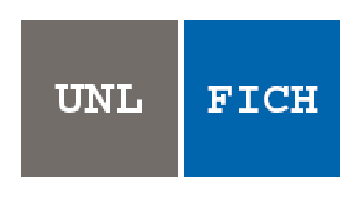
\includegraphics[scale=0.6]{img/fich_unl.eps}}
	\end{figure}
	
  	{Ingeniería Informática}\\
  	{Facultad de Ingeniería y Ciencias Hídricas}\\
    {UNIVERSIDAD NACIONAL DEL LITORAL}	
\end{center}

\bigskip
\bigskip

\newpage

\pagestyle{plain}

\section{Justificación}
Las imágenes y videos presentes en el mundo digital, combinados con la potencialidad que ofrecen los ordenadores 
actuales, han hecho más fácil la creación de aplicaciones sofisticadas en el área de procesamiento de imágenes y visión computacional \cite{citeulike:9456628}.

Desde hace tiempo, los sistemas de realidad aumentada (AR o Augmented Reality) y reconocimiento de objetos,
han pasado a ser un tema pujante en el área de visión computacional, tomando gran 
interés en la comunidad científica y viéndose esto reflejado en diversidad de aplicaciones:
en el área del e-commerce - publicidad  \cite{5478308}, robótica \cite{Chen_markerlessaugmented, conf/icra/2010}, juegos \cite{5711053,Azuma:2001:RAA:616073.618862}, libros interactivos \cite{KimPW09},
industria \cite{conf/visapp/BenhimaneNGGNM08}; en diferentes ambientes \cite{conf/ismar/KleinM07, Chen_markerlessaugmented, Takacs:2008:OAR:1460096.1460165, conf/ismar/MiyashitaMTOESGGAL08}; aplicable sobre diferentes objetos 
\cite{conf/ismar/2007, Lepetit:2005:MMT:1166405.1166406, conf/iswc/2007}; y llevada a cabo mediante el uso de distintos dispositivos \cite{WagnerRMDS10}.

Un sistema de AR reemplaza parte del mundo real con objetos virtuales (generados por computadoras), los cuales parecen coexistir en el mismo espacio que el ambiente real. 
Si bien existen ampliaciones a esta definición, se puede definir a un sistema AR como aquel que posee las siguientes propiedades \cite{Azuma:2001:RAA:616073.618862}:
\begin{itemize}
 \item combina objetos virtuales y reales en un mismo ambiente,
 \item trabaja interactivamente y en tiempo real y,
 \item registra (alinea) objetos reales y virtuales entre sí.
\end{itemize}

La habilidad de reconocer e identificar objetos como imágenes, texto, logos, etc. en una imagen o vídeo para luego ser usados como ``patrones'', es esencial en 
aplicaciones de AR, además de ser usada en control de calidad, vigilancia e identificación visual \cite{5739718}.
%y es por ello que en este trabajo nos centraremos en este tema.

Existe una distinción en realidad aumentada entre dos tipos de sistemas \cite{1320421}: 
\begin{itemize}
 \item los que usan marcadores (\textbf{Marker based}), en los cuales se identifica un ``marcador artificial'' colocado en el ambiente, y por ende alterando el mismo y,
 \item los que no usan marcadores (\textbf{Markerless}), que se sustentan en usar características naturales para identificar objetos del mundo real, es decir, que no usan un ``marcador artificial'' para asistir al reconocimiento del objeto.
\end{itemize}
En ambos casos, el objeto 2D o 3D virtual da la apariencia de aparecer ``pegado'' al marcador o a la característica natural cuando se ve a través del viewport de AR.

De la misma forma, para la detección y seguimiento del objetos, existen diferentes métodos \cite{1320421}, entre los cuales se pueden nombrar:
\begin{itemize}
 \item seguimiento basado en localización (\textbf{location based tracking}): involucra sensores como GPS, acelerómetros, giroscopios, etc. para identificar el objeto y su posición (por lo general menos precisos).
 \item sistemas de reconocimiento (\textbf{optical tracking}): contrariamente a los anteriores, se basa en el análisis e identificación de características a partir de la imagen que permitan identificar y obtener la posición del objeto  (por lo general más precisos).
 \item una combinación de los dos anteriores.
\end{itemize}

En este trabajo nos enmarcaremos en sistemas de realidad aumentada sin marcadores o \textbf{Markerless} y con detección y seguimiento de objetos que no involucren sensores, 
es decir, \textbf{optical tracking}.

Así, se propone construir un método con las características anteriormente nombradas, que permita reconocer objetos planos e identificar su 
posición respecto a una cámara web, en un ambiente controlado, para la posterior aplicación de realidad aumentada. 

El desarrollo de un motor propio de AR que sea fácilmente adaptable a aplicaciones específicas (comerciales, educativas, lúdicas, etc.) resulta de 
gran interés propio y para el grupo, ya  que si bien se puede encontrar software ya desarrollado, no todos trabajan en tiempo real, otros son distribuidos 
bajo licencias privativas o son del tipo Marker based, entre otras características que no lo hacen de interés para su uso. Además, se estaría trabajando 
en una tecnología de punta que se encuentra en auge en estos tiempos y con un futuro prospero. Una de las piezas fundamentales del motor citado, son los métodos de identificación y reconocimiento de objetos los cuales serán expuestos en el presente trabajo. 

Para ello, será necesario aplicar conocimientos de visión computacional \cite{citeulike:3484001, citeulike:9456628, bb1919} e investigar métodos de 
extracción de características en imágenes \cite{Nixon:2002:FEI}. Existen gran cantidad de investigaciones en el área, tales como:
\begin{itemize}
 \item el estudio de descriptores visuales \cite{BouGar} y locales \cite{bb53077, TuytelaarsM07, BenhimaneNGGNM08}, entre los cuales se encuentran los algoritmos SURF (Speeded-Up Robust Features) \cite{Bay:2008:SRF, Bay:2008:SRF} y SIFT (Scale Invariante Feature Transform) \cite{bb48614},
 \item el reconocimiento de puntos claves \cite{bb36798},
 \item la detección en tiempo real de objetos \cite{conf/cvpr/HinterstoisserLIFN10},
 \item el seguimiento (tracking) sin marcadores \cite{5607509},
 \item el análisis de características invariantes en imágenes \cite{conf/ismar/2004, Lowe2004} y
 \item la clasificación de puntos característicos \cite{oai:infoscience.epfl.ch:52666}, entre otros.
\end{itemize}
Dichos temas, se tratarán de abordar en menor o mayor medida para el correcto desarrollo del presente proyecto.

\section{Objetivos}
\subsection{Objetivo general}
  \begin{itemize}
      \item Desarrollar un método para reconocer y seguir objetos en una secuencia de vídeo digital y desarrollar un prototipo que haga uso del mismo.
      \item Afianzar y extender los conocimientos adquiridos en el cursado de la carrera Ingeniería en Informática.
  \end{itemize}
\subsection{Objetivos específicos}
% poner objetivos medibles
\begin{itemize}
	\item Realizar el relevamiento del estado del arte en métodos utilizados para la detección y seguimiento de objetos en el Procesamiento Digital de imágenes.
	\item Desarrollar un método reconocedor y seguidor de objetos planos en el flujo de video tomado por una cámara web estándar, sobre un ambiente controlado.
	\item Implementar el método en un algoritmo computacional que pueda ser utilizado en diferentes sistemas operativos.
	\item Optimizar el método desarrollado para que sea aplicable en tiempo real.
	\item Implementar una aplicación prototipo específica (en el área de turismo, educación, publicidad, juegos u otras) aplicando el método desarrollado.
\end{itemize}

\section{Alcance}
Entre los alcances del proyecto se pueden enumerar los siguientes:
\begin{itemize}
  \item El trabajo se enmarcará en un sistema del tipo Markerless con método de reconocimiento del tipo optical tracking.
  \item El proyecto involucra el desarrollo de un prototipo para ser utilizado en una computadora con una cámara web standard. 
	Cabe aclarar, que no se pretende realizar una aplicación final específica y completa orientada a un usuario final.
  \item Se trabajará con imágenes que conformen un flujo de video en tiempo real capturado por una cámara web de computadora en un ambiente específico y controlado.
  \item No es un objetivo la implementación de varios métodos y su comparación. Sin embargo, en una etapa previa se evaluarán las características de varios métodos para obtener el que mejor se adecue a los requerimientos.
  \item Se dejará como un trabajo futuro la optimización de velocidad y/o implementación por hardware (procesamiento con GPU).
\end{itemize}

\section{Metodología}
\subsection{Revisión y estado del arte.}
Este proyecto comienza con la revisión bibliográfica y del estado de arte de los métodos disponibles para la extracción de características en imágenes/vídeo, 
que sean útiles para el reconocimiento y seguimiento (tracking) de objetos en tiempo real.

\subsection{Identificación de características en imágenes.}
Posteriormente, se buscará implementar, utilizar y/o adaptar un método o algoritmo, que permita identificar dichas 
características sobre objetos planos. En el proceso de detección, se utilizarán técnicas de procesamiento de imágenes, operaciones 
de transformaciones morfológicas, entre otras.
  
\subsection {Proyección, matching y procesamiento.}
Se procederá con la aplicación de proyecciones y/o transformaciones perspectivas o afines, matching de características entre imágenes u 
otras acciones relacionadas con proyecciones que se evalúen durante el desarrollo y que sean necesarias para obtener la ubicación del objeto.

En esta etapa también se pondrá en consideración la posible implementación de un pre-procesamiento para tratar de mejorar la velocidad del algoritmo.

\subsection {Procedimiento de aplicación y finalización.}
La aplicación del código desarrollado, se hará sobre imágenes capturadas en tiempo real, con una cámara web estándar. El procedimiento tendrá dos pasos principales: en una
primera instancia y como parte del proceso de configuración, se capturará una imagen del objeto a detectar, seguidamente, se capturará flujo de vídeo en tiempo real, 
para ser analizado y así llevar a cabo la detección del objeto y el cálculo de su posición respecto a la cámara.

En lo que respecta a herramientas a utilizar para la codificación, existe variedad de software y librerías para la manipulación de videos e imágenes, sin embargo
OpenCV (Open Source Computer Vision)\footnote[1]{http://SourceForge.net/projects/opencvlibrary} es una librería open source\footnote[2]{http://opensource.org} de 
visión computacional, escrita en C y C++, la cual puede ser ejecutada sobre diferentes sistemas operativos: Linux, Windows y Mac OS X, que ha sido ampliamente 
adoptada como la herramienta para el desarrollo en la comunidad de investigadores y desarrolladores en el campo de visión computacional \cite{citeulike:9456628}, debido
a que fue diseñada para lograr gran eficiencia computacional, haciendo foco en el desarrollo de aplicaciones en tiempo real. Es por ello, que como base para el desarrollo 
del código fuente de nuestro método, se utilizará la citada librería. Además, se considerará la utilización de OpenGL si el proyecto así lo requiriese.

Finalmente y para la conclusión del trabajo, se aplicará el método a un prototipo de aplicación específica.

\section{Plan de trabajo y de tareas propuesto}

\begin{enumerate}
    \item Revisión y estado del arte. \textbf{\textit{(Total final: 75 hs.)}}
      \begin{enumerate}
	Recopilación bibliográfica: 
 	\item técnicas de reconocimiento y seguimiento (tracking) de objetos, \textit{(30 hs.)}
	\item procesamiento de flujo de vídeo, \textit{(10 hs.)}
	\item pre-procesamiento de imágenes, \textit{(10 hs.)}
	\item cálculo de homografías, proyecciones y transformaciones. \textit{(25 hs.)}
      \end{enumerate}
% 	
% 		Las tareas a realizar en esta etapa están relacionadas con el estudio y la comprensión de los siguientes temas:
% 	
% 		\begin{enumerate}
% 		  \item Operaciones morfológicas - Pre-procesamiento\textit{(30 hs.)}
% % 		    \begin{enumerate}
% % 			\item Aplicación de umbral en imágenes. \textit{(10 hs.)}
% % 			\item Erosión y dilatación en imágenes. \textit{(10 hs.)}
% % 			\item Detección de movimiento a través de diferencia de frames. \textit{(10 hs.)}
% % 		    \end{enumerate}
% 		  \item Método de extracción de características en imágenes. \textit{(25 hs.)}
% 		  \item Técnicas de maching de característicias entre imágenes. \textit{(10 hs.)}
% 		  \item Homografía, warping y transformación afín. \textit{(10 hs.)}
% 		\end{enumerate}
	
	\item Identificación de características en imágenes. \textbf{\textit{(Total final: 145 hs.)}}
	  \begin{enumerate} 
	    \item Adquisición de imágenes para formar un conjunto de pruebas que sirva de prototipo. \textit{(5 hs.)}
	    \item Implementación, uso o desarrollo de un método de extracción de características en imágenes. \textit{(Total: 140 hs.)}
	      \begin{itemize}
	       \item Análisis/estudio del método. \textit{(75 hs.)}
	       \item Implementación o uso en el código. \textit{(75 hs.)}
	      \end{itemize}
	  \end{enumerate}


% 		\begin{enumerate}
% 			\item Puntos claves (keypoints) y descriptores. \textit{(40 hs.)}
% 			\item Análisis y aplicación del algoritmo SURF para detección de características.\textit{(70 hs.)}
% 			\item Integración del algoritmo SURF en el algoritmo de detección.\textit{(40 hs.)}
% 		\end{enumerate}
	\item Proyección, matching y procesamiento. \textbf{\textit{(Total final: 90 hs.)}}
	  \begin {enumerate} 
	    \item Matching de características entre imágenes. \textit{(10 hs.)}
	    \item Proyecciones. \textit{(10 hs.)}
	    \item Transformaciones. \textit{(10 hs.)}
	    \item Pre-procesamiento para posibles mejoras de velocidad en tiempo de ejecución. \textit{(30 hs.)} %Algunas de las operaciones posiblemente involucradas en este paso serán
	    \item Análisis homográfico. \textit{(30 hs.)}
	  \end{enumerate}
	
% 	    \begin{enumerate}
% 		\item Algoritmo KNN - k-nearest neighbor algorithm. \textit{(20 hs.)}
% 	    \end{enumerate}

	
	
% 		    \begin{itemize}
% 			\item Erosión, \textit{(10 hs.)}
% 			\item Dilatación, \textit{(10 hs.)}
% 			\item Umbral (threshold), \textit{(10 hs.)}
% 			\item Detección de movimiento (diferencia de imágenes), entre otras. \textit{(10 hs.)}
% 		    \end{itemize}
	
	
% 	    \begin{enumerate}
% 		\item Cómputo de homografía entre dos imágenes. \textit{(30 hs.)}
% 	    \end{enumerate}
	\item Procedimiento de aplicación y finalización. \textbf{\textit{(Total final: 240 hs.)}}
	  \begin{enumerate}
	    \item Superposición de contenido (imágenes o videos) sobre el objeto detectado. \textit{(40 hs.)}
	    \item Redacción del informe final del proyecto. \textit{(200 hs.)}
	  \end{enumerate}
\end{enumerate}
\textbf{Total del plan de trabajo y tareas propuesto: 550 hs.}
\section{Puntos de seguimiento}

Comienzo de actividad: Noviembre de 2011.
 
\begin{enumerate}
	\item Punto de control $n^o\ 1$, diciembre de 2011:
		\begin{itemize}
			\item Informe de la bibliografía consultada (recopilación bibliográfica).
		\end{itemize}
		
	\item Punto de control $n^o\ 2$, febrero de 2011:
		\begin{itemize}
		  \item Adquisición de imágenes (prototipos) para realizar las pruebas.			
		  \item Métodos de extracción de características en imágenes parte 1 (Análisis/estudio del método).
		\end{itemize}
		
	\item Punto de control $n^o\ 3$, marzo de 2012:
		\begin{itemize}
			\item Métodos de extracción de características en imágenes parte 2(Implementación o uso en el código).
			\item Matching de características entre imágenes. %(Algoritmo knn - k-nearest neighbor algorithm).
		\end{itemize}	
	
	\item Punto de control $n^o\ 4$, abril de 2012:
		\begin{itemize}
			\item Pre-procesamiento para lograr posibles mejoras de velocidad, en tiempo de ejecución. 
			\item Análisis homográfico, proyecciones y transformaciones.
			\item Superposición de contenido sobre el objeto detectado.
		\end{itemize}
\end{enumerate}


\section{Cronograma tentativo}
\begin{gantt}[xunitlength=1.5cm,fontsize=\small,titlefontsize=\small,drawledgerline=true]{16}{8}
   \begin{ganttitle}
      \titleelement{2011}{2}
      \titleelement{2012}{6}
    \end{ganttitle}
    
    \begin{ganttitle}
		\titleelement{Nov}{1}		
		\titleelement{Dic}{1}
		\titleelement{Ene}{1}
		\titleelement{Feb}{1}
		\titleelement{Mar}{1}
		\titleelement{Abr}{1}
		\titleelement{May}{1}
		\titleelement{Jun}{1}
    \end{ganttitle}
%\ganttgroup{Punto de control $n^o\ 1$}{1}{2}
%    \ganttbar{Tarea 1}{0.3}{1.2}
     \ganttbar{Tarea 1.a}{0}{0.6}        
     \ganttbar{Tarea 1.b}{0.6}{0.2}
     \ganttbar{Tarea 1.c}{0.8}{0.2}
     \ganttbar{Tarea 1.d}{1}{0.5}
        
%\ganttgroup{Punto de control $n^o\ 2$}{3}{1}    
    \ganttbar{Tarea 2.a}{1.5}{0.0625}
    \ganttbar{Tarea 2.b (parte 1)}{1.5625}{0.9375}


	%\ganttgroup{Punto de control $n^o\ 3$}{4}{1}
        \ganttbar{Tarea 2.b (parte 2)}{2.5}{0,882352941}
	%\ganttbar{Tarea 4}{3.2777777}{0.2222}
	\ganttbar{Tarea 3.a}{3,382352941}{0,117647059}
    
	%\ganttgroup{Punto de control $n^o\ 4$}{5}{2}    
	\ganttbar{Tarea 3.b}{3.5}{0.11666667}
	\ganttbar{Tarea 3.c}{3,6166667}{0.11666667}
	\ganttbar{Tarea 3.d}{3,73333337}{0.3500001}
	\ganttbar{Tarea 3.e}{4,08333347}{0.3500001}
	\ganttbar{Tarea 4.a}{4,43333357}{0.466668}

	\ganttbar{Tarea 4.b}{4.8999}{2.5}
	
\end{gantt}

Cabe aclarar que la Tarea 8 incluye tiempos de redacción (redacciones parciales) durante el desarrollo del proyecto.

\section{Recursos necesarios}

\begin{itemize}
	\item Acceso a Internet.
	\item Material bibliográfico.
	\item PC con cámara web y sistema operativo GNU/Linux.
	\item Software de libre distribución (IDE, compiladores, bibliotecas, control de versiones).
\end{itemize}

Los recursos mencionados anteriormente se encuentran disponibles en el Centro de Investigación en Señales, Sistemas e Inteligencia Computacional (Sinc), donde se lleva a cabo el Proyecto.

\section{Presupuesto}

\begin{tabular}{p{3.3cm} p{5.5cm} c r r l}

	\rowcolor[gray]{0.70} \textbf{Tipo} & \textbf{Detalle} & \textbf{Cant.} & \textbf{P. Unit.} &  \textbf{P. Total}\\ 

	\rowcolor[gray]{0.93} \textit{Librería} & & & & \\ \multirow{5}{*}{} 
	& Resma de hojas blancas A4 & 2 & \$23.00 &\$46.00 \\
	& (Entregables, Informe Proyecto Final y Borradores)&  &  &  \\
	& Anillados & 6 & \$13.00 & \$78.00 \\
	& Lapiceras y lápices & 10 & \$3.75 & \$37.50 \\

	\rowcolor[gray]{0.93} \textit{Fotocopias} & & & & \\ \multirow{1}{*}{} 
	& Material bibliográfico & 3 & \$65.00 & \$195.00 \\	
	
	\rowcolor[gray]{0.93} \textit{Hardware}  & & & & \\ \multirow{3}{*}{} 
	%& Impresora laser & 1 & \$400.00 & \$400.00 \\      
	& Monitor LCD 23 pulgadas & 1 & \$1900.00 & \$1900.00 \\      
	& Notebook con webcam & 1 & \$3500.00 & \$3500.00 \\
	& Webcam externa & 1 & \$150.00 & \$150.00 \\
	
	\rowcolor[gray]{0.93} \textit{Recursos humanos} & & & &\\ \multirow{1}{*}{}
	& Honorarios & 8 & \$3300.00 & \$26400.00\\
	        	
	\rowcolor[gray]{0.93} \textit{Servicios} & & & & \\ \multirow{1}{*}{}
	& Acceso a internet & 8 & \$99.90 & \$799.20 \\

	\rowcolor[gray]{0.93} \textit{Software} & & & & \\ \multirow{1}{*}{} 
	& Ide, librerías, compiladores, control de versión, etc & 1 & \$0.00 & \$0.00 \\	

	\rowcolor[gray]{0.70} & & & \textbf{Total} & \textbf{\$36105.70} \\

\end{tabular}


\begin{itemize}
	\item La totalidad del software utilizado en el proyecto es de distribución libre y gratuita, con lo cual no se aplican gastos de licencias para su uso.
	\item A pesar que el hardware está disponible en el SINC, se incluye en el presupuesto, ya que son recursos utilizados cuando no se está el mismo.
\end{itemize}
\newpage
\bibliographystyle{alpha}
\bibliography{bib1,bib2,bib3,bib4}
\end{document}
